\documentclass[a4paper, 12pt]{report}
\usepackage{graphicx} % Required for inserting images
\usepackage{pdfpages}
\usepackage{amsmath}   % for \text and many math helpers
\usepackage{amssymb}   % for \therefore and other symbols
\usepackage{enumerate}
\usepackage{cancel}
\usepackage{multicol}
\usepackage{lipsum}
\usepackage{pythonhighlight}
\usepackage[margin=2cm]{geometry}
\usepackage{titlesec}
\usepackage{titling}
\newcommand{\subtitle}[1]{%
  \posttitle{%
    \par\end{center}
    \begin{center}\huge#1\end{center}
    \vskip0.5em}%
}
\usepackage{fancyhdr}
\usepackage{lastpage}   
\usepackage{eurosym}
\makeatletter
\renewcommand\chapter{%
    \if@openright\cleardoublepage\else\clearpage\fi% a
%   \thispagestyle{fancy} % not needed <<<<<
    \global\@topnum\z@%
    \@afterindentfalse%
    \secdef\@chapter\@schapter}
\makeatother

\fancypagestyle{frontmatter}{% 
    \fancyhf{}% clear previous definitions
    \pagenumbering{roman}
    \fancyfoot[R]{\thepage}
}

\fancypagestyle{mainmatter}{%
    \fancyhf{}% clear previous definitions
    \pagenumbering{arabic}
    \fancyfoot[R]{Page \thepage\ of \pageref{LastPage}}
}

\renewcommand{\headrulewidth}{0pt}% no upper rule <<<<<
%\renewcommand{\footrulewidth}{0.5pt}% optional foot rule <<<<<

\newcommand{\sectionbreak}{\clearpage}
\pdfminorversion=7
\usepackage{hyperref}
\usepackage[style=apa, backend=biber]{biblatex}

\addbibresource{refs.bib}

\title{GENG4411 Engineering Research Project Part 1 \\ Project Proposal}
\subtitle{\textbf{Assessing climate injustice in the housing market}\vspace{2cm}}
\author{\Large \textbf{Joel Wright}\\23783614\\School of Engineering, University of Western Australia\vspace{2cm}\\\Large \textbf{John Duncan}\\School of Agriculture and Environment, University of Western Australia}
\date{\vfill
\textbf{School of Engineering\\
University of Western Australia\vspace{2cm}}
\\April 2026}

\begin{document}

\pagenumbering{roman}
\pagestyle{frontmatter}

\maketitle
\addcontentsline{toc}{chapter}{Title Page}
\newpage

\chapter*{Signed Declaration}
% Add your signed declaration content here
\addcontentsline{toc}{chapter}{Signed Declaration}
\newpage

\chapter*{Project Summary}
% Add your project summary content here
\addcontentsline{toc}{chapter}{Project Summary}
\newpage

\tableofcontents
\addcontentsline{toc}{chapter}{Table of Contents}

\listoffigures
\addcontentsline{toc}{chapter}{List of Figures}

\listoftables
\addcontentsline{toc}{chapter}{List of Tables}

\chapter*{Nomenclature}
% Add your nomenclature content here
\addcontentsline{toc}{chapter}{Nomenclature}
\newpage

\pagenumbering{arabic}
\pagestyle{mainmatter}

\chapter{Introduction, Literature Review and Project Objectives}
\section{Introduction}
Following the onset of the pandemic, however, the Australian housing
market began experiencing dramatic year-on-year growth, with Western Australia subsequently
recording some of the most significant price increases nationwide \parencite{perth_market_growth}. This rapid escalation has generated widespread concern that housing availability will
not keep pace with demand. As a result, many first-home buyers are committing to increasingly unaffordable loans- according to KPMG modelling, these loans are now being serviced by 31\% of household income, compared with 23\% in 2019/20 \parencite{KPMG2025}. Yet, even with many people maxing out their borrowing capacity, the types of houses they can afford may still be less than desirable. Perth, a hot city, will continue to experience warm summers, Figure \ref{2-week-average-summer-temp} compares the 5 most recent summers with all historical data. How Perth manages future heat stress is uncertain, and housing policy will be influential to an individual's heat exposure.  \begin{figure}[htbp!]
    \centering
    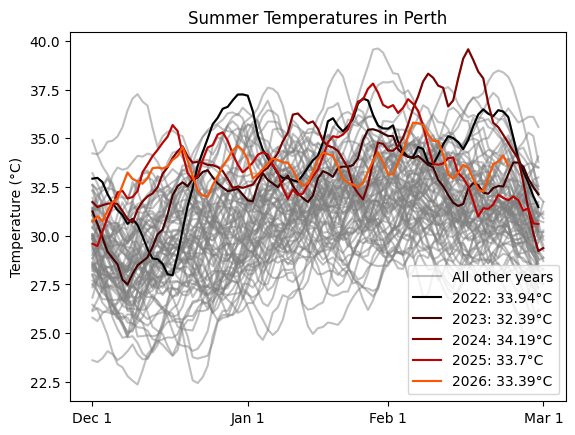
\includegraphics[height=0.5\textwidth]{2-week-average-summer-temp.png}
    \caption{Rolling fortnightly averaged temperatures during Perth summer. Mean temperatures - including the hottest summer (2024) - given. Historical mean = $31.08^{\circ}$C\\ \rightline{Data from \cite{BOM_temps}}}
    \label{2-week-average-summer-temp}
\end{figure}
\section{Literature Review (or Background)}
A literature review will be conducted exploring four areas: \begin{enumerate}
\item How built form responds to baseline and heatwave conditions, (determining whether to use a future climate model)
\item An appropriate methodology for determining air surface temperature and thermal comfort, (Justifying the use of TARGET)
\item Property market trends, (why is this an issue NOW?)
\item The human response to thermal stress, (why should we care?)
\end{enumerate}
\subsection{How built form responds to baseline and heatwave conditions}
Built form - the concentration of buildings, paved surfaces, and other anthropogenic materials within the urban environment - plays a central role in shaping local thermal conditions. When present at sufficient density, these materials contribute to the urban heat island (UHI) effect, as urban areas exhibit systematically higher temperatures than their surrounding rural or less-developed landscapes. In the natural environment, evapotranspiration from vegetation and exposed soils offer environmental cooling. Additionally, the increased heat load from airconditioning exhaust during these periods further contributes to UHI, however this will not be studied further in this project.

In normal conditions, this phenomenon occurs as harsh surfaces with a high volumetric heat capacity like concrete, pavement, and bitumen shift the energy balance such that more heat is absorbed throughout the day \parencite{UHI}. Overnight, this thermal load is released back into the environment, leading to warmer nocturnal temperatures such that the UHI-heatwave interaction is strongest overnight \parencite{UHI_and_extremes}. During heatwaves, the geometries of urban areas further contribute to the entrapment of heat energy - the urban canopy decreases any atmospheric mixing, seen in Figure \ref{urban_canopy}.  \begin{figure}[htbp]
    \centering
    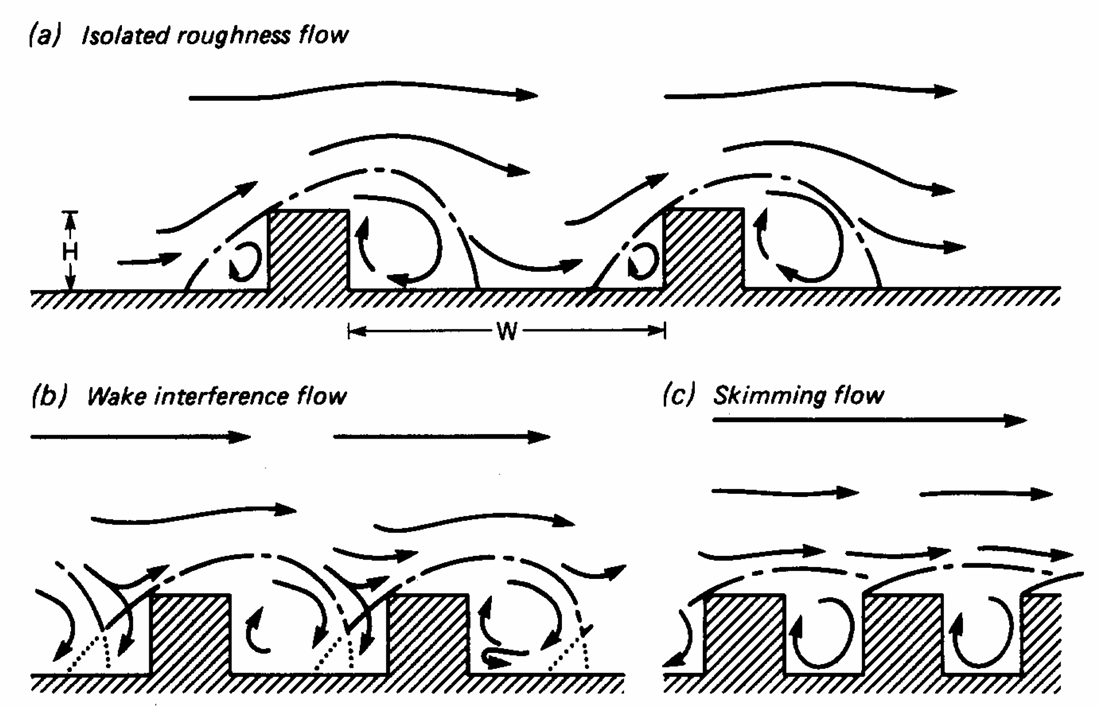
\includegraphics[height=0.5\textwidth]{Urban_canopy.png}
    \caption{Flow regimes over urban canopy \\ \rightline{\parencite{urban-canopy-mixing}}}
    \label{urban_canopy}
\end{figure}

As shown in Figure \ref{2-week-average-summer-temp}, temperatures have been observed to increase over the past several years. Going forward, \cite{Heat_stress_count} predict an increase to days above $35^{\circ}$ (totalling 26, up nine), an increase to days above $40^{\circ}$ (totalling four, up two), and an increase to nights above $25^{\circ}$ (totalling three, up two) by 2050 with current climate change action. Using  future climate modelling as an input into the TARGET model uncovers the benefits of marginal increases to tree canopy cover, as previous studies have shown that the cooling influence of Green/Blue infrastructure is amplified/ ideal for heatwave forcings (\cite{heatwave-cooling}, \cite{TARGET}, \cite{Fast-urban-climate-model-GBI}, \cite{projection_of_heatwaves}). Climate change is a global problem and for this reason, many feel hopelessness towards their own actions \parencite{Climate-despair}, however, with the increased sensitivity to marginal land cover changes discussed previously, individuals can improve their own environment.   
\subsection{An appropriate methodology for determining air surface temperature and thermal comfort}
There are many options for finding air temperatures in an urban environment, this section will step through each of their utility,
\subsubsection{Satellite sensing} Satellites can only measure the surface temperature of surfaces they see (JOHN HAS SOURCE). Land surface temperature (LST) data from the most common satellite remote sensing project - Moderate Resolution Imaging Spectroradiomter (MODIS) - has a resolution of $500m/250m$ \parencite{LST_res}, compared to the block-scale ($20m\times 20m$) of the study. Further, in a study of the dynamics of LST and air temperature, it was found that the conditions of this study do not lend to LST being an appropriate proxy for air temperature \parencite{LST-TA}.
\subsubsection{Weather stations}
The Perth metro region has a network of publicly funded weather stations from the Bureau of Meteorology (BoM) and Department of Primary Industry and Regional Development available \parencite{agricDPIRDWeather}, as well as a network of citizen weather stations \parencite{netatmoWeathermap}. These stations offer insight into the climate of the greater Perth region, however their density is not sufficient to measure block-scale microclimates. Likewise, the locations of the commercial weather stations - typically in isolated areas, away from urban areas \parencite{BoM-guidelines} - does not allow comparisons between built form. 
\subsubsection{Sensors}
Another option for observing urban microclimates is the deployment of dense networks of in-situ temperature sensors at targeted locations. For example, a London-based study deployed 39 sensors across parks and built-up areas to compare air temperature and thermal comfort conditions \parencite{london-study}. Each sensor cost approximately \euro 335 and required calibration, installation, monitoring, and retrieval, a significant investment of both time and resources.

Beyond financial and labour constraints, sensor-based approaches are also subject to systematic location biases. Sensors must be mounted on existing infrastructure such as light poles, traffic signs, or buildings, and their placement is contingent on approval from the relevant authority; It is unlikely homeowners would allow sensors located inside their property. Scaling this approach to the scope of this study ($n = 50,000$), is therefore unfeasible.
\subsubsection{Advanced models}
(CHECK WITH JOHN)
\subsubsection{TARGET}
The Air-temperature Response to Green/blue Infrastructure Evaluation Tool (TARGET) offers reduced-complexity modelling of near-surface air temperature in the urban environment \parencite{TARGET}. It produces parcel-scale outputs (approximately $50$--$150\,\text{m} \times 50$--$150\,\text{m}$ resolution) using site-specific land-cover data (REF NEARMAP). This allows simulations to extend across both public and private land, incorporating their respective surface characteristics into energy balance calculations.

Although TARGET was originally developed and validated for Melbourne \parencite{TARGET}, literature treats Melbourne comparably with Perth \parencite{Perth-Melbourne}. Additionally, it has subsequently been shown TARGET is suitable for other urban contexts \parencite{Fast-urban-climate-model-GBI}. By building on the Local-Scale Urban Meteorological Parameterisation Scheme (LUMPS) \parencite{LUMPS}, the model captures key surface-atmosphere interactions without the risk of over-parameterisation. TARGET is therefore well suited to short-duration studies and permits the use of heatwave and future climate forcings, enabling consistent comparison across baseline and projected climate conditions. This Project will also validate TARGET's use in Perth?? 
\subsection{Property market trends}

\subsection{The human response to thermal stress}
The idea that the environment fundamentally influences the human experience and human behaviours has been circulating since Ancient Greece, Rome, and imperial China - Hippocrates argued that factors like climate and topology have a profound impact on the physiology and health of native peoples; Confucius believed in strong linkages between Heaven, Earth, and Humanity. It should be no surprise that extreme hot temperatures and heatwave cause exacerbated rates of heat stress and higher rates of mortality. In fact it is the number-one cause of weather-related deaths globally; In June-August of 2003, 70,000 people died in a European heatwave event \parencite{WHO}. The extent to which other human outcomes are also influenced by increased heat-exposure is discussed in \parencite{Social-economic} which cites many studies that have found some link between climate variables and social and economic outcomes - increased temperature correlates to increased instances of aggression and conflict (\cite{Hsiang2011-db}; \cite{climate-on-conflict}; \cite{temperature-temperament}; \cite{Crime-weather}); decreased mathematics testing performance (NOT TRUE FOR ENGLISH/READING) (\cite{child-test-scores}), and decreased labour performance in high-risk industries (defined as agriculture, forestry, fishing, and hunting; mining; construction; manufacturing; and transportation and utilities industries.) \parencite{temp-labour}; GDP, productivity and income (\cite{US-income}; \cite{Temp-GDP}; \cite{Temp-production}). While these studies don't have Perth or Australian regions of interest and one could argue that a Perth population must have some higher level of tolerance to heat exposure due to climate adaptation, \parencite{Adjusted-pops} found that mortality rates during days over $35^{\circ}$, the mortality rate increases in Cold, Temperate, and Hot climates.

\section{Project Objectives}
Key discoveries that need to be made to prove/disprove the hypothesis

Where this project fall in to literature (Currently there is lots of talk about both climate resilience and housing affordability, there is limited papers linking them (some talk about extreme whether events). This paper will drive a strong link for "normal conditions")
\chapter{Project Process}
\section{Modelling Investigations}
Modelling investigations often include model derivation and then implementation using a software package or written code.  For modelling investigations this section might include:\begin{itemize}

\item Model derivation (or modification) 
\item A description and diagram of the model configuration
\item A description of any software tools / platforms to be used and/or created and reason(s) for choice
\item Descriptions of the model input options to be considered (boundary conditions, constitutive behaviours, etc)
\item A description of any model validation tests that will be done, i.e., how will you check that your model is producing or will produce reliable and accurate results?
\item What are the model’s limitations?
\end{itemize}

\chapter{Timeline and Risk Management}
Identify critical paths and dominoes in it. 

Risks - installing/removing sensors, reliance on additional (discretional) funding... 
\chapter{Progress to Date}

% https://github.com/Joel-does-code/Thesis_Assignment-Latex/blob/main
\printbibliography
\end{document}